\documentclass{article}
\usepackage{booktabs}
\usepackage{makecell}
\usepackage{multirow}
\usepackage{fullpage}
\usepackage{csvsimple}
\usepackage{setspace}
\usepackage{graphicx}
\usepackage{tabularx}

\title{FIN9013 Assignment 1}
\author{Ang Zhang}

\begin{document}
\maketitle

\singlespacing

\section*{Introduction}
This report examines the determinants of the debt ratio of firms using a panel data of 16,257 observations.
The data management step processed the data by defining the dependent variable, $Debt$, as the total debt over total book asset.
The independent variables include the logarithm of annual sales turnover, $Size$, the market to book ratio of assets, $MB$,
and a dummy variable indicating whether the firm has R\&D spending, $D(RD)$.
Varies models, including linear models and discrete choice models are used to examine the relationshio.
To account for the potential endogeneity of the MB variable, instrument variables is introduced and
validated through two stage LS. Then, panel data estimation is performed to account for
heterogeneity (potential correlation between the error terms across firms/years).

Moving on, treatment effect is studied with DD analysis to examine a shock to a subset of the firms
located in a specific region. Matching model is also used to estimate the treatment effect which shows similar results.

The report is organized as follows: Table 1 in appendix presents summary statistics for the variables used in the analysis.
Each section presents the results of the different models used in the analysis, with detailed results
presented in tables in the appendix.

\section*{Linear regression, interactions, split-samples and non-linearities}
In this section, a total of seven linear regression models are estimated. Generally, the \textit{Size} variable has a positive
effect on the debt ratio, while the \textit{MB} variable has a negative effect. The \textit{D(RD)} variable has a negative effect
on the debt ratio, which suggests that firms with R\&D spending have a lower debt ratio than firms without R\&D spending.
In the split sample model where only firms with R\&D spending are included, the \textit{MB} variable is not significant.
\begin{equation}
    Debt = \beta_0 + \beta_{size} Size + \beta_{mb} MB + \beta_{rd} D(RD) + \epsilon_{it}
\end{equation}
In the baseline model of \textit{eq.1}, the slope term of $Size$ factor is 0.0237,
which means that for a one unit increase in the logarithm of annual sales turnover,
measured in millions, the predicted value of the debt ratio, measured by the total debt over total book asset, \
increase by 0.0237, holding all other variables constant.
The slope term of $MB$ factor is 0.0033, which means that for a one unit increase in the market to book ratio of assets,
the predicted value of the debt ratio, measured by the total debt over total book asset, \
increase by 0.0033, holding all other variables constant.
The slope term of $D(RD)$ factor is -0.0771, which means that for a firm with positive R\&D spending,
the predicted value of the debt ratio, measured by the total debt over total book asset, \
is 0.0771 lower than a comparable firm with no R\&D spending, holding all other variables constant.

In the baseline model, when holding all variables at their mean ,the predicted \textit{Debt} is 0.197 while for all variables at their median,
the predicted \textit{Debt} is 0.172. Since there's no interaction term in \textit{eq.1}, the effect of $D(RD)$ on \textit{Debt} is constant
at -0.0033, no matter where $MB$ stands at. The coefficient of $D(RD)$ solely determines the effect that $D(RD)$ has on \textit{Debt}.

However, we can hardly say that this model is a good fit, as the $R^2$ value is only 0.1054, which means that only 10.54\% of the
variation in the dependent variable, $Debt$, can be explained by the independent variables, $Size$, $MB$ and $D(RD)$,
while the rest 89.46\% of the variation is due to other factors not included in the model.

\begin{equation}
    Debt = \beta_0 + \beta_{size} Size + \beta_{mb} MB + \beta_{rd} D(RD) + \beta_{mbrd} MB \cdot D(RD) + \epsilon_{it}
\end{equation}

In \textit{eq.2}, the added interaction term is also statistically significant at 1\% level. Predicted \textit{Debt} is 0.194
when all predictors are held at their mean, while it is 0.168 when all predictors are held at their median. For the a firm at 25-th
percentile of $MB$, the effect of $D(RD)$ on \textit{Debt} is -0.091, while for a firm at 75-th percentile of $MB$, the effect of $D(RD)$ on \textit{Debt} is
-0.064. This suggests that \textit{D(RD)} affect firms with different market to book ratio in different ways.

In the split sample model, in firms with positive R\&D spending we still observe the \textit{Size} effect but this time we don't
observe the \textit{MB} effect. The coefficient for \textit{MB} is not significant event at 10\% level. For firms with no R\&D spending,
both explanatory variables are still significant.

In the augmented model where both interaction terms are included, all coefficients are significant at 1\% level.
Specifically, in this augmented model if we hold D(RD) euqal to 1, the effects of \textit{Size} and \textit{MB} alignes well with
the split sample model where only firms with R\&D spending are included. Same is also true if we hold D(RD) equal to 0 and compare to the
split sample model with only firms without R\&D spending.

In the RD rank model, the coefficient for the RD rank variable is not significant even at 10\% level. This is conterintuitive
as previously we have already observed the singificant role that R\&D spending plays in determining the debt ratio of firms.
This means a plain RD rank variable didn't catch the dynamics of the R\&D spending, and that it is very likely that the effect of R\&D spending
is non-linear. Looking at the RD class model where RD rankk is included as a categorical variable (dummy encoded),
all resulting categorical variables are significant at 1\% level. This confirms that the effect of R\&D spending is non-linear.

Comparing all models, the RD class model has the highest $R^2$ value of 0.1253, which means it's a better fit.
Albeit from this, the $R^2$ value is still low, which means that the model still cannot explain a large portion of the variation a firm's debt ratio.

Detailed results are presented in Table 2 in the appendix.

\section*{Discrete choice variables and censoring}
In this section, a total of five discrete choice models are estimated. The logit model and probit model are estimated with and without interaction terms.
The Tobit model is also estimated. All coefficients are significant at 1\% level.
The coefficients here, however, are not comparable to the linear regression models, because instead of pointing to the change in the dependent variable,
they point to the change in the link function, which is the logit function in logit regression and the normal CDF in probit regression.
For the model estimated with eq.1, predicted \textit{Debt} is 0.314 when all predictors are held at their mean, while it is 0.286 when all predictors are held at their median.
When all variables held at their median, margianl effects of \textit{Size}, \textit{MB} and \textit{D(RD)} are 0.0561, -0.0226 and -0.1220 respectively.
Marginal effect of D(RD) is -0.1247 for a firm with \textit{MB} at 25-th percentile, while it is -0.1164 for a firm with \textit{MB} at 75-th percentile.
For the model estimated with eq.2, predicted \textit{Debt} is 0.307 when all predictors are held at their mean, while it is 0.276 when all predictors are held at their median.

The discrete choice model built-in the statsmodel package do offer a marginal effect function (get\_margeff) to calculate the
marginal effect of the independent variables. But the question with this package is that it cannot account for interaction terms.
The reason is that in statsmodel package, the model takes each interaction term as a separate variable, so the marginal effect
function cannot calculate the marginal effect of the interaction term. But for logit model, the marginal effect can be calculated
manually by taking the derivative of the probability function with respect to the independent variable and there's a closed-form solution as below:
\begin{equation}
    \frac{\partial P(Debt|D(RD))}{\partial D(RD)} = (\beta_{rd} + \beta_{mbrd} MB ) \cdot P(y=1|x) \cdot (1-P(y=1|x))
\end{equation}
where $P(y=1|x)$ is the estimated logic probability, at the point where the marginal effect is to be calculated.
For the model estiamted with eq.2, marginal effects of \textit{Size}, \textit{MB} and \textit{D(RD)} are 0.0564, -0.0069 and -0.1298 respectively.
Marginal effect of D(RD) is -0.1521 for a firm with \textit{MB} at 25-th percentile, while it is -0.0860 for a firm with \textit{MB} at 75-th percentile.
Although the estimated coefficients are different for the logit and probit models, the marginal effects are similar. The predicted value at
the same points are also similar for the logit and probit models.

The Python statsmodel package does not have a Tobit model specification as with the Logit and Probit, so I manually defined a class to estimate the Tobit model.
The model class inherits from the statsmodel GLM class, and the log-likelihood function is defined as the sum of the log-likelihood of the
censored and uncensored observations.

Although the resutls in the discrete choice models are not directly comparable with the linear models in Table 2,
the direction to which the coefficents point to and whether they are significant should be consistent, given the monotonic characteristic of the link function.
And the results are also the case.

Detailed results are presented in Table 3 in the appendix.

\section*{Instrumental variables}
For an instrument to be valid, it must be correlated with the endogenous variable, \textit{MB},
but uncorrelated with the error term. The first assumption is tested by regressing \textit{MB} on the instrument and look at the statistics
including R-squared and F-statistics. Here first stage results shows significance in coefficience of D(DecIPO) at 1\% level, and the
F-stats of 412 is also much larger than the rule-of-thumb cutoff of 10. However the R-squared value is only 0.071, which I will doubt if
the instrument is strong enough.

But the second assumption cannot be tested directly, because the endogenous variable
have distorted the error term so that the error term is no longer a "real" error term.
But we can use economic intuition to think about whether the instrument is likely to be correlated with the error term.
Heuristically, which month did the firm go public is unlikely to be correlated with the debt ratio, because the month of the IPO
is unlikely to have any effect on the how much debt the firm decides to take on.
But a firm that goes public in December may face significantly different market conditions
when many investors are on vacation, thus may experience a dip in their valuation, thus negatively impacting
their market value. Even though market condition would revert, the initial market perception of the firm
would continue to be at play and exibits a path dependence which persistently play a part in the firms's market value.

Detailed resutls are presented in Table 4 in the appendix.

\section*{Panel data estimation}
The resuls for panel data estimation with firm-level fixed effects and random effects are consistent with the OLS, the only thing in that
significance level of \textit{MB} dropped. However,
whehn year fixed-effects are included, the coefficient of \textit{MB} become insiginificant.
The agumented model with \textit{D(DecIPO)} shows insiginificant coefficient for this added dummy variable when combined with RE,
and when firm-level fixed effects are included, the Python package was unable to estimate D(DecIPO).
That is expected because the IPO month of a firm is either in December or not in December, so
this dummy variable is absorbed by the fixed effects of the firm.

Detailed results are presented in Table 5 in the appendix.

\section*{DD analysis}
The baseline model shows a positive coefficient for \textit{D(Post)} and a negative coefficient for
\textit{D(Treated)}, while controlling for Size, MB, and D(RD). That means for comparable firms from NY/CA versus from other
stats, the debt ratio on average for the former is lower than the latter. The coefficient of \textit{D(Post)} is
positive, which means that the debt ratio for firms in NY/CA increases after the treatment.

When firm fixed-effect is introduced, the variable \textit{D(Treated)} is fully
absorbed because a firm is either in NY/CA or not, unless the firm has moved either from NY/CA to other states or
from other states to NY/CA. With both firm fixed effects and year fixed effects, both \textit{D(Treated)} and \textit{D(Post)} are absorbed
because again, \textit{D(Treated)} only depends on the year which is absorbed into year FE. In all three models, the interaction
term between \textit{D(Treated)} and \textit{D(Post)} is insignificant.
When examining the set of indicators for each year together with \textit{D(Treated)}, a clear trend can be spotted.
Recall that key identifying assumption of DD is “Parallel Trends”, which stipulates that no correlation between outcome
and assignment, and that in absence of treatment, the outcome for treated and controls is unaffected.
From Figure \ref{fig:parallel_trends}, we can see that the trend of the debt ratio for the treated group and the control group
is parallel before the treatment, which is the year 2000. After the treatment, the debt ratio for the treated group increases more than the trend
suggested by the control group. This suggests that the treatment has a positive effect on the debt ratio of the treated group.
This is also consistent with the coefficients in the baseline model.

\begin{figure}[h!]
    \centering
    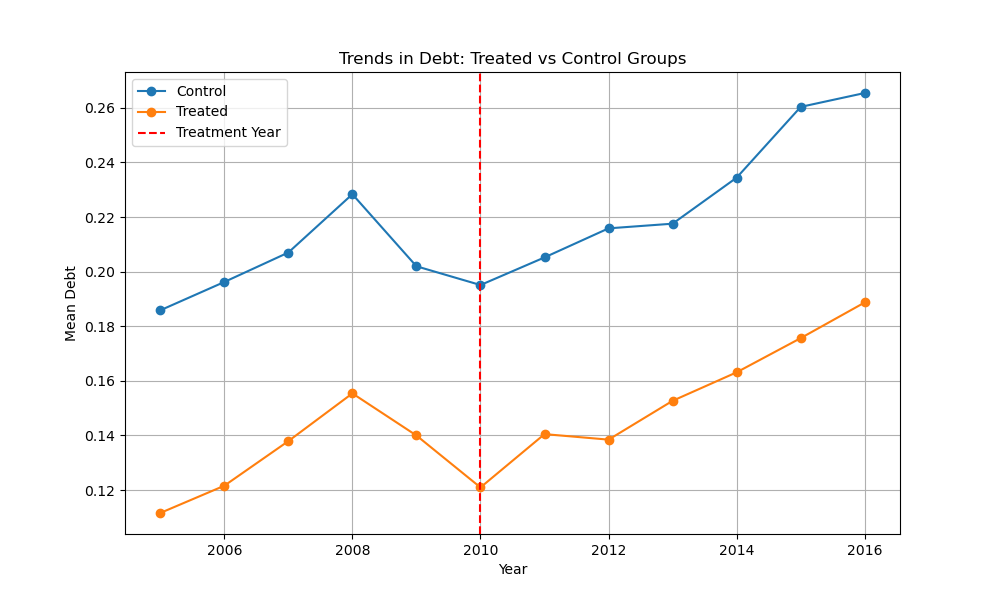
\includegraphics[width=0.8\textwidth]{parallel_trends.png}
    \caption{Parallel Trends Assumption}
    \label{fig:parallel_trends}
\end{figure}

Detailed results are presented in Table 6 in the appendix.

\section*{Matching models}
In year 2010 only, the coefficient of \textit{D(Treated)} is -0.049 and significant at 5\% level, which (may) suggest that
firms in NY/CA that are affected by the shock have a lower debt ratio than firms in other states. This is consistent with the DD analysis.
With propensity score matching, the coefficient of \textit{D(Treated)} is -0.039 and significant at 5\% level.
This suggests that the treatment effect is robust. The implication of the matching model is that for firm with close probability
of receiving treatment based on their \textit{Size}, \textit{MB}, and \textit{D(RD)}, the treated firm exhibits a lower debt ratio
than their "matches" in other states. This is consistent with the DD analysis and the baseline model.
Using a nearest neighbor matching of 2 neighors give a similar result, with the coefficience of \textit{D(Treated)} of -0.043
and again significant at 5\% level. This suggests that the treatment effect is robust to the choice of the number of neighbors.

Detailed results are presented in Table 7 in the appendix.

\section*{Appendix}

\begin{table}[h!]
    \centering
    \caption{Summary Statistics Table}
    \label{table:1}
    \begin{tabular}{lcccccccc}
        \toprule
        \multicolumn{8}{c}{Panel A: All Firms}                                        \\
        \midrule
        Variable  & N     & Mean  & StdDev & Min    & P25   & Median & P75   & Max    \\
        \midrule
        Debt      & 16257 & 0.197 & 0.225  & 0      & 0.000 & 0.129  & 0.317 & 1.017  \\
        Size      & 16257 & 5.786 & 2.060  & -0.997 & 4.576 & 5.991  & 7.194 & 10.068 \\
        MB        & 16257 & 1.912 & 1.549  & 0.334  & 0.923 & 1.397  & 2.344 & 8.834  \\
        D\_RD     & 16257 & 0.582 & 0.493  & 0      & 0     & 1.000  & 1.000 & 1.000  \\
        RD\_rank  & 16257 & 1.908 & 1.120  & 1.000  & 1.000 & 2.000  & 2.000 & 5.000  \\
        D\_Debt   & 16257 & 0.336 & 0.472  & 0      & 0     & 0      & 1.000 & 1.000  \\
        D\_DecIPO & 16257 & 0.089 & 0.285  & 0      & 0     & 0      & 0     & 1.000  \\
        \midrule
        \multicolumn{8}{c}{Panel B: Firms with R\&D}                                  \\
        \midrule
        Variable  & N     & Mean  & StdDev & Min    & P25   & Median & P75   & Max    \\
        \midrule
        Debt      & 9468  & 0.150 & 0.201  & 0      & 0     & 0.058  & 0.246 & 1.017  \\
        Size      & 9468  & 5.183 & 2.168  & -0.997 & 3.908 & 5.299  & 6.658 & 10.068 \\
        MB        & 9468  & 2.202 & 1.699  & 0.334  & 1.064 & 1.644  & 2.760 & 8.834  \\
        D\_RD     & 9468  & 1.000 & 0      & 1.000  & 1.000 & 1.000  & 1.000 & 1.000  \\
        RD\_rank  & 9468  & 2.559 & 1.068  & 2.000  & 2.000 & 2.000  & 3.000 & 5.000  \\
        D\_Debt   & 9468  & 0.245 & 0.430  & 0      & 0     & 0      & 0     & 1.000  \\
        D\_DecIPO & 9468  & 0.079 & 0.270  & 0      & 0     & 0      & 0     & 1.000  \\
        \midrule
        \multicolumn{8}{c}{Panel C: Firms without R\&D}                               \\
        \midrule
        Variable  & N     & Mean  & StdDev & Min    & P25   & Median & P75   & Max    \\
        \midrule
        Debt      & 6789  & 0.264 & 0.239  & 0      & 0.049 & 0.226  & 0.401 & 1.017  \\
        Size      & 6789  & 6.626 & 1.548  & -0.997 & 5.686 & 6.647  & 7.689 & 10.068 \\
        MB        & 6789  & 1.508 & 1.199  & 0.334  & 0.807 & 1.140  & 1.748 & 8.834  \\
        D\_RD     & 6789  & 0     & 0      & 0      & 0     & 0      & 0     & 0      \\
        RD\_rank  & 6789  & 1.000 & 0      & 1.000  & 1.000 & 1.000  & 1.000 & 1.000  \\
        D\_Debt   & 6789  & 0.463 & 0.499  & 0      & 0     & 0      & 1.000 & 1.000  \\
        D\_DecIPO & 6789  & 0.103 & 0.304  & 0      & 0     & 0      & 0     & 1.000  \\
        \bottomrule
    \end{tabular}
    \newline
    \textit{Note: This table presents the summary statistics for the variables used in the analysis. Panel A includes all firms, Panel B includes firms with R\&D, and Panel C includes firms without R\&D.}
\end{table}

\begin{table}[h!]
    \centering
    \caption{Parameter Estimates of Each Model}
    \label{table:2}
    \begin{tabular}{lccccccc}
        \toprule
        Parameter  & \makecell{Model                                                                                                               \\ Baseline} & \makecell{Model \\ Interaction} & \makecell{Model \\ Augmented} & \makecell{Model \\ RD} & \makecell{Model \\ No RD} & \makecell{Model \\ RD Rank} & \makecell{Model \\ RD Class} \\
        \midrule
        Intercept  & \makecell{0.1114***                                                                                                           \\ (0.0068)} & \makecell{0.1298*** \\ (0.0072)} & \makecell{0.1029*** \\ (0.0119)} & \makecell{0.0292*** \\ (0.0063)} & \makecell{0.1029*** \\ (0.0131)} & \makecell{0.0376*** \\ (0.0090)} & \makecell{0.1070*** \\ (0.0071)} \\
        Size       & \makecell{0.0237***                                                                                                           \\ (0.0009)} & \makecell{0.0242*** \\ (0.0009)} & \makecell{0.0282*** \\ (0.0017)} & \makecell{0.0227*** \\ (0.0009)} & \makecell{0.0282*** \\ (0.0018)} & \makecell{0.0297*** \\ (0.0010)} & \makecell{0.0334*** \\ (0.0010)} \\
        MB         & \makecell{-0.0033***                                                                                                          \\ (0.0011)} & \makecell{-0.0175*** \\ (0.0022)} & \makecell{-0.0173*** \\ (0.0022)} & \makecell{0.0015 \\ (0.0012)} & \makecell{-0.0173*** \\ (0.0024)} & \makecell{-0.0072*** \\ (0.0012)} & \makecell{-0.0067*** \\ (0.0011)} \\
        D\_RD      & \makecell{-0.0771***                                                                                                          \\ (0.0037)} & \makecell{-0.1092*** \\ (0.0055)} & \makecell{-0.0737*** \\ (0.0137)} & & & \\
        MB*D\_RD   &                      & \makecell{0.0194***                                                                                    \\ (0.0025)} & \makecell{0.0188*** \\ (0.0025)} & & & \\
        Size*D\_RD &                      &                     & \makecell{-0.0055***                                                             \\ (0.0020)} & & & \\
        RD\_rank   &                      &                     &                      &        &        & \makecell{0.0008                        \\ (0.0020)} &  \\
        RD\_rank 1 &                      &                     &                      &        &        &                  & \makecell{-0.0547*** \\ (0.0081)} \\
        RD\_rank 2 &                      &                     &                      &        &        &                  & \makecell{-0.1358*** \\ (0.0076)} \\
        RD\_rank 3 &                      &                     &                      &        &        &                  & \makecell{-0.1473*** \\ (0.0097)} \\
        RD\_rank 4 &                      &                     &                      &        &        &                  & \makecell{-0.0337**  \\ (0.0158)} \\
        \midrule
        RSquare    & 0.1054               & 0.1086              & 0.1091               & 0.0586 & 0.0419 & 0.0809           & 0.1253               \\
        \#Obs      & 16257                & 16257               & 16257                & 9468   & 6789   & 16257            & 16257                \\
        \bottomrule
    \end{tabular}
    \newline
    \textit{Note: This table presents the parameter estimates for various models.
        The baseline model includes the intercept, Size, and MB.
        The interaction model adds an interaction term between MB and D\_RD.
        The augmented model includes additional interaction terms.
        The RD model includes only firms with R\&D, while the No RD model includes firms without R\&D.
        The RD Rank model includes the RD\_rank variable,
        and the RD Class model includes categorical variables for RD\_rank.
        Standard errors are in parentheses.
        Significance levels are indicated by * p\textless 0.1, ** p\textless 0.05, *** p\textless 0.01.}
\end{table}

\begin{table}[h!]
    \centering
    \caption{Limited Dependent Variable Models}
    \label{table:3}
    \begin{tabular}{lccccc}
        \toprule
                  & (1) Logit & (2) Logit+Int & (3) Probit & (4) Probit+Int & (5) Tobit \\
        \midrule
        Intercept & -1.811*** & -1.630***     & -1.058***  & -0.941***      & 0.1113*** \\
                  & (0.077)   & (0.081)       & (0.045)    & (0.047)        & 0.007     \\
        Size      & 0.275***  & 0.280***      & 0.158***   & 0.161***       & 0.024***  \\
                  & (0.010)   & (0.010)       & (0.006)    & (0.006)        & (0.001)   \\
        MB        & -0.111*** & -0.259***     & -0.055***  & -0.151***      & -0.003*** \\
                  & (0.013)   & (0.024)       & (0.008)    & (0.014)        & (0.001)   \\
        D\_RD     & -0.598*** & -0.963***     & -0.371***  & -0.598***      & -0.077*** \\
                  & (0.037)   & (0.059)       & (0.022)    & (0.035)        & (0.004)   \\
        MB×D\_RD  &           & 0.224***      &            & 0.138***       &           \\
                  &           & (0.029)       &            & (0.016)        &           \\
        \bottomrule
    \end{tabular}
    \newline
    \textit{Note: Standard errors are in parentheses. Significance levels are indicated by * p\textless 0.1, ** p\textless 0.05, *** p\textless 0.01.
        (1)Logit model is the logistic regression model for eq.1, (2) Logit + Int is the logistic regression model for eq.2 with interaction term,
        (3) Probit model is the probit regression model for eq.1, (4) Probit + Int is the probit regression model for eq.2,
        (5) Tobit model is the Tobit regression model for eq.1.}
\end{table}

\begin{table}[h!]
    \centering
    \caption{Two-Stage Least Squares (2SLS) Analysis}
    \label{table:4}
    \begin{tabular}{lcc}
        \toprule
        Variables         & First Stage (MB)  & Second Stage (Debt) \\
        \midrule
        Intercept         & 2.284*** (0.044)  &                     \\
        Size              & -0.114*** (0.006) &                     \\
        D\_RD             & 0.525*** (0.025)  &                     \\
        D\_DecIPO[T.True] & -0.223*** (0.041) &                     \\
        \midrule
        const             &                   & 0.250*** (0.065)    \\
        Size              &                   & 0.017*** (0.003)    \\
        MB                &                   & -0.065** (0.029)    \\
        D\_RD             &                   & -0.044*** (0.016)   \\
        \midrule
        R-squared         & 0.071             & -0.061              \\
        N                 & 16257             & 16257               \\
        F-statistic       & 412.16            &                     \\
        \bottomrule
    \end{tabular}
    \newline
    \textit{Note: Standard errors are in parentheses. Significance levels are indicated by * p\textless 0.1, ** p\textless 0.05, *** p\textless 0.01.}
\end{table}

\begin{table}[h!]
    \centering
    \caption{Panel Data Estimations (Fixed Effects and Random Effects)}
    \begin{tabular}{lccccccc}
        \toprule
        Variables & OLS       & FE        & RE        & FE Year   & RE Year   & FE Augmented & RE Augmented \\
        \midrule
        Intercept & 0.111***  & 0.062***  & 0.084***  & 0.114***  & 0.084***  & 0.062***     & 0.084***     \\
                  & (0.007)   & (0.012)   & (0.010)   & (0.012)   & (0.010)   & (0.012)      & (0.010)      \\
        Size      & 0.024***  & 0.027***  & 0.027***  & 0.018***  & 0.027***  & 0.027***     & 0.027***     \\
                  & (0.001)   & (0.002)   & (0.001)   & (0.002)   & (0.001)   & (0.002)      & (0.001)      \\
        MB        & -0.003*** & -0.002**  & -0.002**  & -0.001    & -0.002**  & -0.002**     & -0.002**     \\
                  & (0.001)   & (0.001)   & (0.001)   & (0.001)   & (0.001)   & (0.001)      & (0.001)      \\
        D\_RD     & -0.077*** & -0.028*** & -0.059*** & -0.032*** & -0.059*** & -0.028***    & -0.059***    \\
                  & (0.004)   & (0.009)   & (0.006)   & (0.009)   & (0.006)   & (0.009)      & (0.006)      \\
        D\_DecIPO &           &           &           &           &           &              & 0.005        \\
                  &           &           &           &           &           &              & (0.014)      \\
        \bottomrule
    \end{tabular}
    \newline
    \textit{Note: Standard errors are in parentheses. Significance levels are indicated by * p\textless 0.1, ** p\textless 0.05, *** p\textless 0.01.}
\end{table}

\begin{table}[h!]
    \centering
    \caption{Difference-in-Differences Analysis}
    \label{table:5}
    \begin{tabular}{lcccc}
        \toprule
        Variables                   & (1) Baseline        & (2) Firm FE & (3) Firm+Year FE & (4) Dynamic         \\
        \midrule
        D\_Post                     & \makecell{0.024***                                                         \\ (0.005)}  & \makecell{0.011** \\ (0.005)} &                  &                   \\
        D\_Treated                  & \makecell{-0.046***                                                        \\ (0.011)} &                 &                  &                   \\
        D\_Post\_x\_Treated         & \makecell{0.003                                                            \\ (0.010)}     & \makecell{0.014 \\ (0.010)}   & \makecell{0.014 \\ (0.010)}    &                   \\
                                    &                     &             &                  & \makecell{-0.071*** \\ (0.015)} \\
        D\_Treated\_x\_year\_2005.0 &                     &             &                  & \makecell{-0.064*** \\ (0.014)} \\
        D\_Treated\_x\_year\_2006.0 &                     &             &                  & \makecell{-0.051*** \\ (0.014)} \\
        D\_Treated\_x\_year\_2007.0 &                     &             &                  & \makecell{-0.041*** \\ (0.014)} \\
        D\_Treated\_x\_year\_2008.0 &                     &             &                  & \makecell{-0.052*** \\ (0.013)} \\
        D\_Treated\_x\_year\_2009.0 &                     &             &                  & \makecell{-0.070*** \\ (0.012)} \\
        D\_Treated\_x\_year\_2010.0 &                     &             &                  & \makecell{-0.059*** \\ (0.011)} \\
        D\_Treated\_x\_year\_2011.0 &                     &             &                  & \makecell{-0.051*** \\ (0.011)} \\
        D\_Treated\_x\_year\_2012.0 &                     &             &                  & \makecell{-0.036*** \\ (0.011)} \\
        D\_Treated\_x\_year\_2013.0 &                     &             &                  & \makecell{-0.025*** \\ (0.010)} \\
        D\_Treated\_x\_year\_2014.0 &                     &             &                  & \makecell{-0.014*   \\ (0.007)}   \\
        D\_Treated\_x\_year\_2015.0 &                     &             &                  & NaN                 \\
        \midrule
        R-squared                   & 0.116               & 0.021       & 0.008            & 0.025               \\
        N                           & 16257               & 16257       & 16257            & 16257               \\
        \bottomrule
    \end{tabular}
    \newline
    \textit{Note: Standard errors are in parentheses. Significance levels are indicated by * p\textless 0.1, ** p\textless 0.05, *** p\textless 0.01.}
\end{table}

\begin{table}[h!]
    \centering
    \caption{Cross-sectional Analysis with Matching (Year 2010)}
    \label{table:6}
    \begin{tabular}{lccc}
        \toprule
        Variables  & (1) OLS             & (2) PSM (n=5) & (3) PSM (n=2) \\
        \midrule
        const      & \makecell{0.120***                                  \\ (0.022)}  & \makecell{0.095*** \\ (0.023)} & \makecell{0.125*** \\ (0.026)}  \\
        D\_Treated & \makecell{-0.049***                                 \\ (0.012)} & \makecell{-0.039** \\ (0.016)} & \makecell{-0.043*** \\ (0.013)} \\
        Size       & \makecell{0.021***                                  \\ (0.003)}  & \makecell{0.025*** \\ (0.003)} & \makecell{0.019*** \\ (0.003)}  \\
        MB         & \makecell{-0.007**                                  \\ (0.004)}  & \makecell{-0.009* \\ (0.005)}  & \makecell{-0.005 \\ (0.004)}    \\
        \bottomrule
    \end{tabular}
    \newline
    \textit{Note: Standard errors are in parentheses. Significance levels are indicated by * p\textless 0.1, ** p\textless 0.05, *** p\textless 0.01.}
\end{table}

\end{document}